\documentclass[10pt,twocolumn]{article}

\usepackage[utf8]{inputenc}
\usepackage[T1]{fontenc}
\usepackage{times}
\usepackage[margin=0.8in,columnsep=0.3in]{geometry}
\usepackage{amsmath,amssymb}
\usepackage{booktabs}
\usepackage{array}
\usepackage{graphicx}
\usepackage{enumitem}
\usepackage{microtype}
\usepackage[hidelinks]{hyperref}

\setlist{nosep,leftmargin=*}
\setlength{\abovecaptionskip}{4pt}
\setlength{\belowcaptionskip}{0pt}

% Rupee amounts: the simulator works in pounds, and every amount below is
% converted at 1 GBP = 105 INR. "Rs." keeps the file compilable with plain pdfLaTeX.
\newcommand{\Rs}{\mbox{Rs.}\,}
\newcommand{\lakh}{\,lakh}

\title{\textbf{Explainable Supply Chain Optimization:\\
Reinforcement Learning Against Tuned Classical Policies,\\
with a Number-Checked Language-Model Explainer}}

\author{%
  Koushik \quad Santosh \quad Srinith \quad Dharani Pratap\\[4pt]
  Amrita Vishwa Vidyapeetham, Coimbatore\\[2pt]
  CB.SC.U4AIE23312 \quad CB.SC.U4AIE23310 \quad CB.SC.U4AIE23357 \quad CB.SC.U4AIE23330}
\date{}

\begin{document}
\maketitle

% ------------------------------------------------------------------ abstract
\begin{abstract}
\noindent
Every day a retailer has to decide how much of each product to order and which
supplier to use. We built a decision-support system for this problem and tested
a reinforcement learning agent against four classical inventory policies that
we tuned ourselves. The system has a simulator calibrated on 1,067,371 real
sales records, a MaskablePPO agent that picks quantity and supplier together,
the four classical policies, and a language model that explains each decision
and also writes crisis scenarios for testing. Every method was scored on the
same 30 held-out simulation runs.

The tuned agent earns \Rs 79.7\lakh{} per 180-day run. That is 90.8\% of the
best classical policy (\Rs 87.8\lakh{}), and it beats two of the four classical
policies. The gap to the best one is modest but real (paired $t=-6.45$,
$n=30$, 95\% CI 5.5 to 10.6\lakh{}). Most of it comes from ordering fees: the
agent splits its orders across suppliers and pays about twice as much in fees,
and nothing in its inputs tells it what it ordered earlier. Action masking made
the agent about three times better, and tuning closed 38\% of the gap that was
left. Training on LLM-written crises did not make the agent more robust
($t=+1.69$, not significant), while plain tuning did. For the explainer, 5 of
30 raw LLM outputs contained a number the simulator never produced. A number
check caught all five, which lifts the accuracy of what the user sees from 83\%
to 100\%.
\end{abstract}

% ------------------------------------------------------------------ 1 intro
\section{Introduction}

A shop that orders badly loses money in two different ways. If it orders too
much, cash sits in the warehouse, storage costs add up, and seasonal items end
up unsold. If it orders too little, customers go elsewhere and the sale is
gone. Choosing a supplier makes this harder. One supplier is cheap but slow,
one is quick but expensive, and a third looks fine on paper but ships only 80\%
of what was asked for and goes offline more often than the others. Since
today's order turns into next week's stock, each decision changes the
situation for the next one.

The usual tools here are rules like $(s,S)$, EOQ with a reorder point, the
newsvendor model, and forecasting with safety stock. They look at one product
at a time and assume demand behaves reasonably. In our data it does not: the
variance of daily demand is about 216 times its mean, much more than a Poisson
model would give. Reinforcement learning (RL) can in principle learn a combined
ordering and sourcing policy that no simple formula captures, and earlier work
has tried deep RL on inventory problems with mixed results against tuned rules
\cite{gijsbrechts,beer}. There is also a practical problem. A buyer is unlikely
to follow a recommendation that nobody can explain.

We wanted to check two things: whether an RL agent can match or beat tuned
classical policies, and whether an LLM can make the agent's decisions
understandable without inventing facts. We kept the baselines strong, kept the
test runs separate from everything used for tuning, and decided in advance to
report the result whichever way it came out. This paper makes the following
contributions.
\begin{enumerate}
  \item A complete system with a calibrated simulator, a MaskablePPO agent that
    chooses quantity and supplier jointly, four tuned classical baselines, an
    LLM explainer, an LLM crisis generator, and a recommend-only dashboard
    (Sections 3--5).
  \item A fair comparison on 30 held-out runs with paired tests. The tuned
    agent reaches 90.8\% of the best classical policy, and the remaining
    \Rs 8.1\lakh{} gap can be traced to one specific cause (Sections 6.1
    and 7).
  \item Two controlled ablations. Action masking is worth about $3\times$ and
    tuning closes 38\% of what is left, but training on LLM-generated crises
    does not improve robustness (Sections 6.2 and 6.3).
  \item A measurement of the explainer showing that its number check matters:
    83\% of raw outputs were correct, against 100\% of delivered ones
    (Section 6.4).
\end{enumerate}

% --------------------------------------------------------------- 2 related
\section{Related Work}

\paragraph{Deep RL for inventory.}
Oroojlooyjadid et al.\ \cite{beer} trained a deep Q-network on the beer game
and found it matched or beat base-stock policies when the players cooperate.
That game has one product in a serial chain and no choice of supplier.
Gijsbrechts et al.\ \cite{gijsbrechts} used an actor-critic method on
lost-sales and dual-sourcing problems. It came out about as good as well-tuned
heuristics, not clearly better, and it needed a lot of tuning. Boute et al.\
\cite{boute} review the field and list fair benchmarking and interpretability
among the open problems. Our setting adds the joint choice of quantity and
supplier under one shared warehouse, and we treat fair benchmarking as a
requirement of the study.

\paragraph{Policy optimization and action masking.}
Proximal Policy Optimization \cite{ppo} limits how far each update can move the
policy and is a common stable default. Huang and Ontañón \cite{masking} showed
that masking invalid actions is a valid policy-gradient method and works with
large action spaces. This is what makes our daily action space of
$21^{10}\approx 1.7\times10^{13}$ combinations manageable. We build on the
Stable-Baselines3 library \cite{sb3}.

\paragraph{Retail demand data.}
Chen et al.\ \cite{chen} applied data mining to online-retail transactions of
the same kind as the UCI Online Retail II set \cite{uci} that we use.

\paragraph{Explanation.}
A trained policy outputs a number and no reason, which is one reason such
policies rarely reach a decision-maker. We do not try to open the network.
The LLM only restates facts that the simulator computed, and a check rejects
any number it makes up (Section 4.4). As far as we know, an RL inventory agent,
a number-checked LLM explainer, and an LLM that writes the test scenarios have
not been evaluated together before. We claim this only for our own setting.

% ------------------------------------------------------------- 3 task setup
\section{Problem Setup}

\paragraph{Data.}
The UCI Online Retail II dataset \cite{uci} has 1,067,371 sales records from a
UK online gift shop. We removed cancelled orders, returns, negative quantities
and rows with no product code, and summed the sales into one row per product
per day. Saturdays are left out because the shop never traded on them, and
filling them with zeros would create a weekly dip that is not real. We picked
ten products on purpose so that they cover three kinds of demand: four steady
ones (coefficient of variation 1.02 to 1.20), three moderate ones (1.29 to
1.65) and three bursty ones (2.09 to 2.34). The agent never sees the raw
records. We measure five things from them (mean demand, variability, weekday
pattern, month pattern and how often a day has no sales), and the simulator
recreates demand from those with a Gamma--Poisson (negative binomial) model.

\paragraph{Environment.}
The environment is a Gymnasium simulator with 10 products, 3 suppliers and
180 days per run. The first 14 days are a warm-up and are not scored. All
products share one warehouse of 20,000 units, and any delivery that does not
fit is refused and written off. A day runs in this order: deliveries arrive,
demand is drawn (adjusted for weekday and month), sales are made, orders are
placed, and profit is counted. Unmet demand becomes a lost sale with a penalty
and is carried over as backlog. Orders come after demand because a real buyer
places them once the day is known. Stock left at the end is valued at 60\% of
its cost, and storage costs 0.15\% of item cost per day. The suppliers
(Table~\ref{tab:suppliers}) are our own invention, because no public dataset
records supplier terms. None of them is better than the others on every count.

\begin{table}[t]
\centering\small
\setlength{\tabcolsep}{3pt}
\begin{tabular}{lcccc}
\toprule
Supplier & Price & Lead & Ships & Fee \\
\midrule
EconoSource & base & 5--8 d & 90\% & \Rs 2,100 \\
RapidTrade  & +35\% & 1--3 d & 98\% & \Rs 4,725 \\
MidWay      & +15\% & 3--5 d & 80\% & \Rs 3,150 \\
\bottomrule
\end{tabular}
\caption{The three suppliers. Minimum orders are 100, 20 and 50 units. MidWay
goes offline most often and RapidTrade almost never.}
\label{tab:suppliers}
\end{table}

\paragraph{Decision and objective.}
Each day, for each product, the system picks one of $7\times3=21$ options:
a quantity level and a supplier. Across 10 products that is
$21^{10}\approx1.7\times10^{13}$ combinations per day. The aim is to maximise
profit,
\begin{equation}\begin{split}
\text{profit}={}&\text{sales}-\text{purchases}-\text{storage}\\
&-\text{fees}-\text{stockout}-\text{overflow}.
\end{split}\end{equation}

\paragraph{Seed groups.}
We use three separate groups of random seeds. Seeds 100 to 111 tune the
classical policies, seeds 900 to 905 pick the best checkpoint during training,
and seeds 500 to 529 are used only for the final numbers. On each of those
final seeds every method sees the same customers and the same delivery delays,
so comparisons are paired.

\paragraph{Metrics.}
Profit optimisation has no ground-truth label, so classification accuracy does
not apply. We report mean profit per 180-day run, relative profit (the agent's
profit divided by the best classical profit), fill rate (the share of demand
served), and the ordering, stockout and overflow costs. For the explainer we
report \emph{raw accuracy} (every number real and all key details present) and
\emph{delivered accuracy} (after the number check).

% ------------------------------------------------------------------ 4 method
\section{Method}

\subsection{System Overview}

The system has five parts: the simulator, a MaskablePPO agent, four tuned
classical policies, an LLM explainer and an LLM crisis generator. A Streamlit
dashboard ties them together in what we call shadow mode. The best classical
policy is the \emph{engine}. The agent runs next to it as a \emph{challenger}
that is scored but never acts. Any decision can be explained on request. The
dashboard only recommends and never places an order.

\subsection{Agent and Objective}

The agent sees 88 numbers. For each product these are stock on hand, stock on
order, days of cover, the 7-day mean and variability of demand, the demand
trend and the backlog. On top of that come the weekday, the time of year, and
each supplier's availability, lead time and recent reliability. The action is a
vector of ten entries, one per product, each over the 21 joint options.
Quantity and supplier are chosen together rather than separately. This trained
$2.8\times$ faster, and it matches how the decision works, since a large order
only makes sense from a supplier that can deliver it. The reward is the day's
profit, scaled and clipped, and it is zero during the warm-up.

We use MaskablePPO. PPO maximises the clipped surrogate objective
\begin{equation}
L^{\text{CLIP}}(\theta)=\hat{\mathbb{E}}_t\!\left[\min\!\big(\rho_t\hat A_t,\;
\text{clip}(\rho_t,1-\epsilon,1+\epsilon)\hat A_t\big)\right],
\end{equation}
where $\rho_t=\pi_\theta(a_t|s_t)/\pi_{\theta_\text{old}}(a_t|s_t)$. Masking
adds a vector $m$ to the logits $z$ before the softmax,
\begin{equation}
\pi_\theta(a\mid s)=\operatorname{softmax}(z+m)_a,\quad
m_a=\begin{cases}0&\text{legal}\\-\infty&\text{illegal,}\end{cases}
\end{equation}
so an offline supplier or an order too large for the warehouse can never be
sampled. The network is small (two layers of 128 or 256 units) and trains on a
CPU.

\subsection{Classical Baselines}

We implemented four textbook policies that choose from the same 21 options per
product as the agent, so none of them has finer control than the others:
$(s,S)$, EOQ with a reorder point, the newsvendor model, and forecasting with
safety stock. Each was tuned with a grid search on the 12 tuning seeds. This
step matters. Widening the search lifted the best policy from \Rs 69.7\lakh{}
to \Rs 89.2\lakh{} on the tuning seeds, and an untuned baseline would have made
the agent look better than it is.

\subsection{LLM Explainer and the Number Check}

We never ask the LLM why a decision was made. The agent's real reason sits
inside a neural network, so any ``because'' from the LLM would be a plausible
story and not the cause. Instead the LLM is given a set of facts $F$ that the
simulator computed (stock, orders in transit, days of cover, recent demand,
what was ordered and from whom, and that supplier's lead time and reliability)
and writes two or three sentences from them. Let $N(x)$ be the set of numbers
in a text $x$. We accept the output $y$ only if $N(y)\subseteq N(F)$ and the key
details are present. Otherwise a fixed template is shown. Three free models are
tried in turn (\texttt{gemma-4-31b-it}, \texttt{glm-5.2},
\texttt{nemotron-3-ultra-550b-a55b}) through OpenRouter, with retries, because
the free endpoints often hit rate limits.

\subsection{Crisis Generator and Training on Crises}

We ask the LLM for realistic supply-chain crises. It returns scenarios such as a
demand spike on four products, a supplier outage, a delivery delay and a cost
increase, and these overlap in time. We do not trust the output. The scenario
type has to be one we know, supplier and product numbers have to exist (invalid
product numbers are dropped, not wrapped around), values are clamped to safe
ranges, and the time window is moved inside the 180 days. We tested this with
six deliberately broken inputs, and each was either corrected or rejected.

For training on crises we saved 16 crisis sets built from 19 scenarios and
split them 10 for training and 6 for testing. At the start of each run the agent
trains on a random set from the training part, and it is tested only on the 6
it has never seen. Its seed, settings and number of steps match the untuned
agent, so crisis exposure is the only difference.

% --------------------------------------------------------- 5 experimental
\section{Experimental Setup}

\paragraph{Training.}
All agents use MaskablePPO. The untuned agent trains for 1M steps with default
settings. For the hyperparameter search we ran eight configurations for 250,000
steps each, then trained the best two to 2M steps on Kaggle. Each long run took
about 1.5 hours, and the whole search about 4.8 hours. Table~\ref{tab:hparams} lists the winning configuration. Checkpoints
are chosen on seeds 900 to 905 and results come from seeds 500 to 529.

\begin{table}[t]
\centering\small
\begin{tabular}{lc}
\toprule
Setting & Value \\
\midrule
Learning rate & $5\times10^{-5}$ (lowest offered) \\
Entropy coefficient & 0.005 \\
Discount $\gamma$ & 0.995 \\
Rollout length & 1024 \\
Network & $[256,256]$ \\
Training steps & 2M \\
\bottomrule
\end{tabular}
\caption{Winning hyperparameters from the 8-configuration search.}
\label{tab:hparams}
\end{table}

The search picked the lowest learning rate and the larger network. That fits
what we suspected: the earlier runs were unstable because they learned too
fast, and the network size was not the problem.

\paragraph{Training logs.}
Figure~\ref{fig:term-train} shows the console output of a short 30,000-step
training run, which we made only to show what the training console reports. The
models reported in this paper were trained for 1M and 2M steps. Under it,
Figure~\ref{fig:term-hist} shows the checkpoint evaluations printed for the
tuned 2M-step run, and Figure~\ref{fig:term-sweep} shows the summary of the
hyperparameter search.

\begin{figure*}[t]
\centering
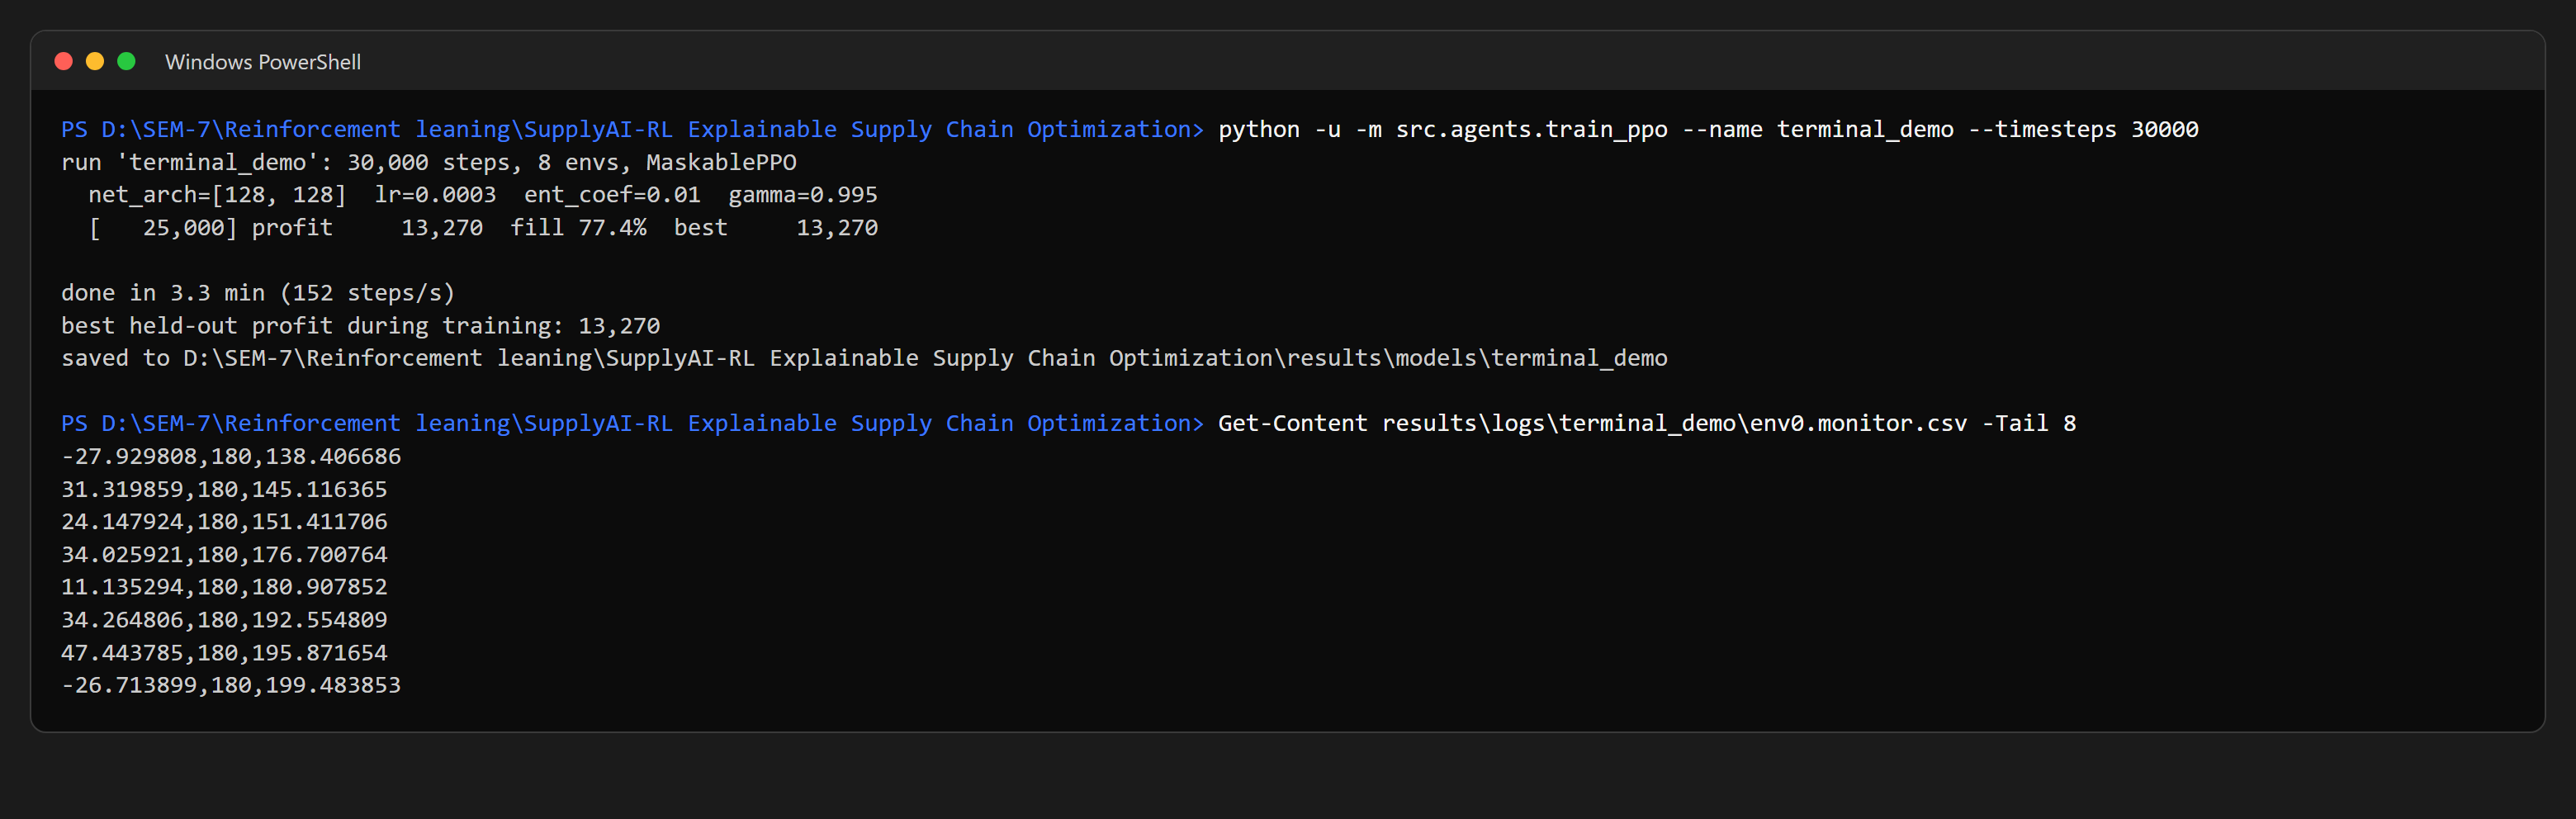
\includegraphics[width=0.92\textwidth]{figures/terminal_train.png}
\caption{Terminal output of a short training run (30,000 steps) with the
project's training script. The reported models were trained for 1M and 2M
steps.}
\label{fig:term-train}
\end{figure*}

\begin{figure*}[t]
\centering
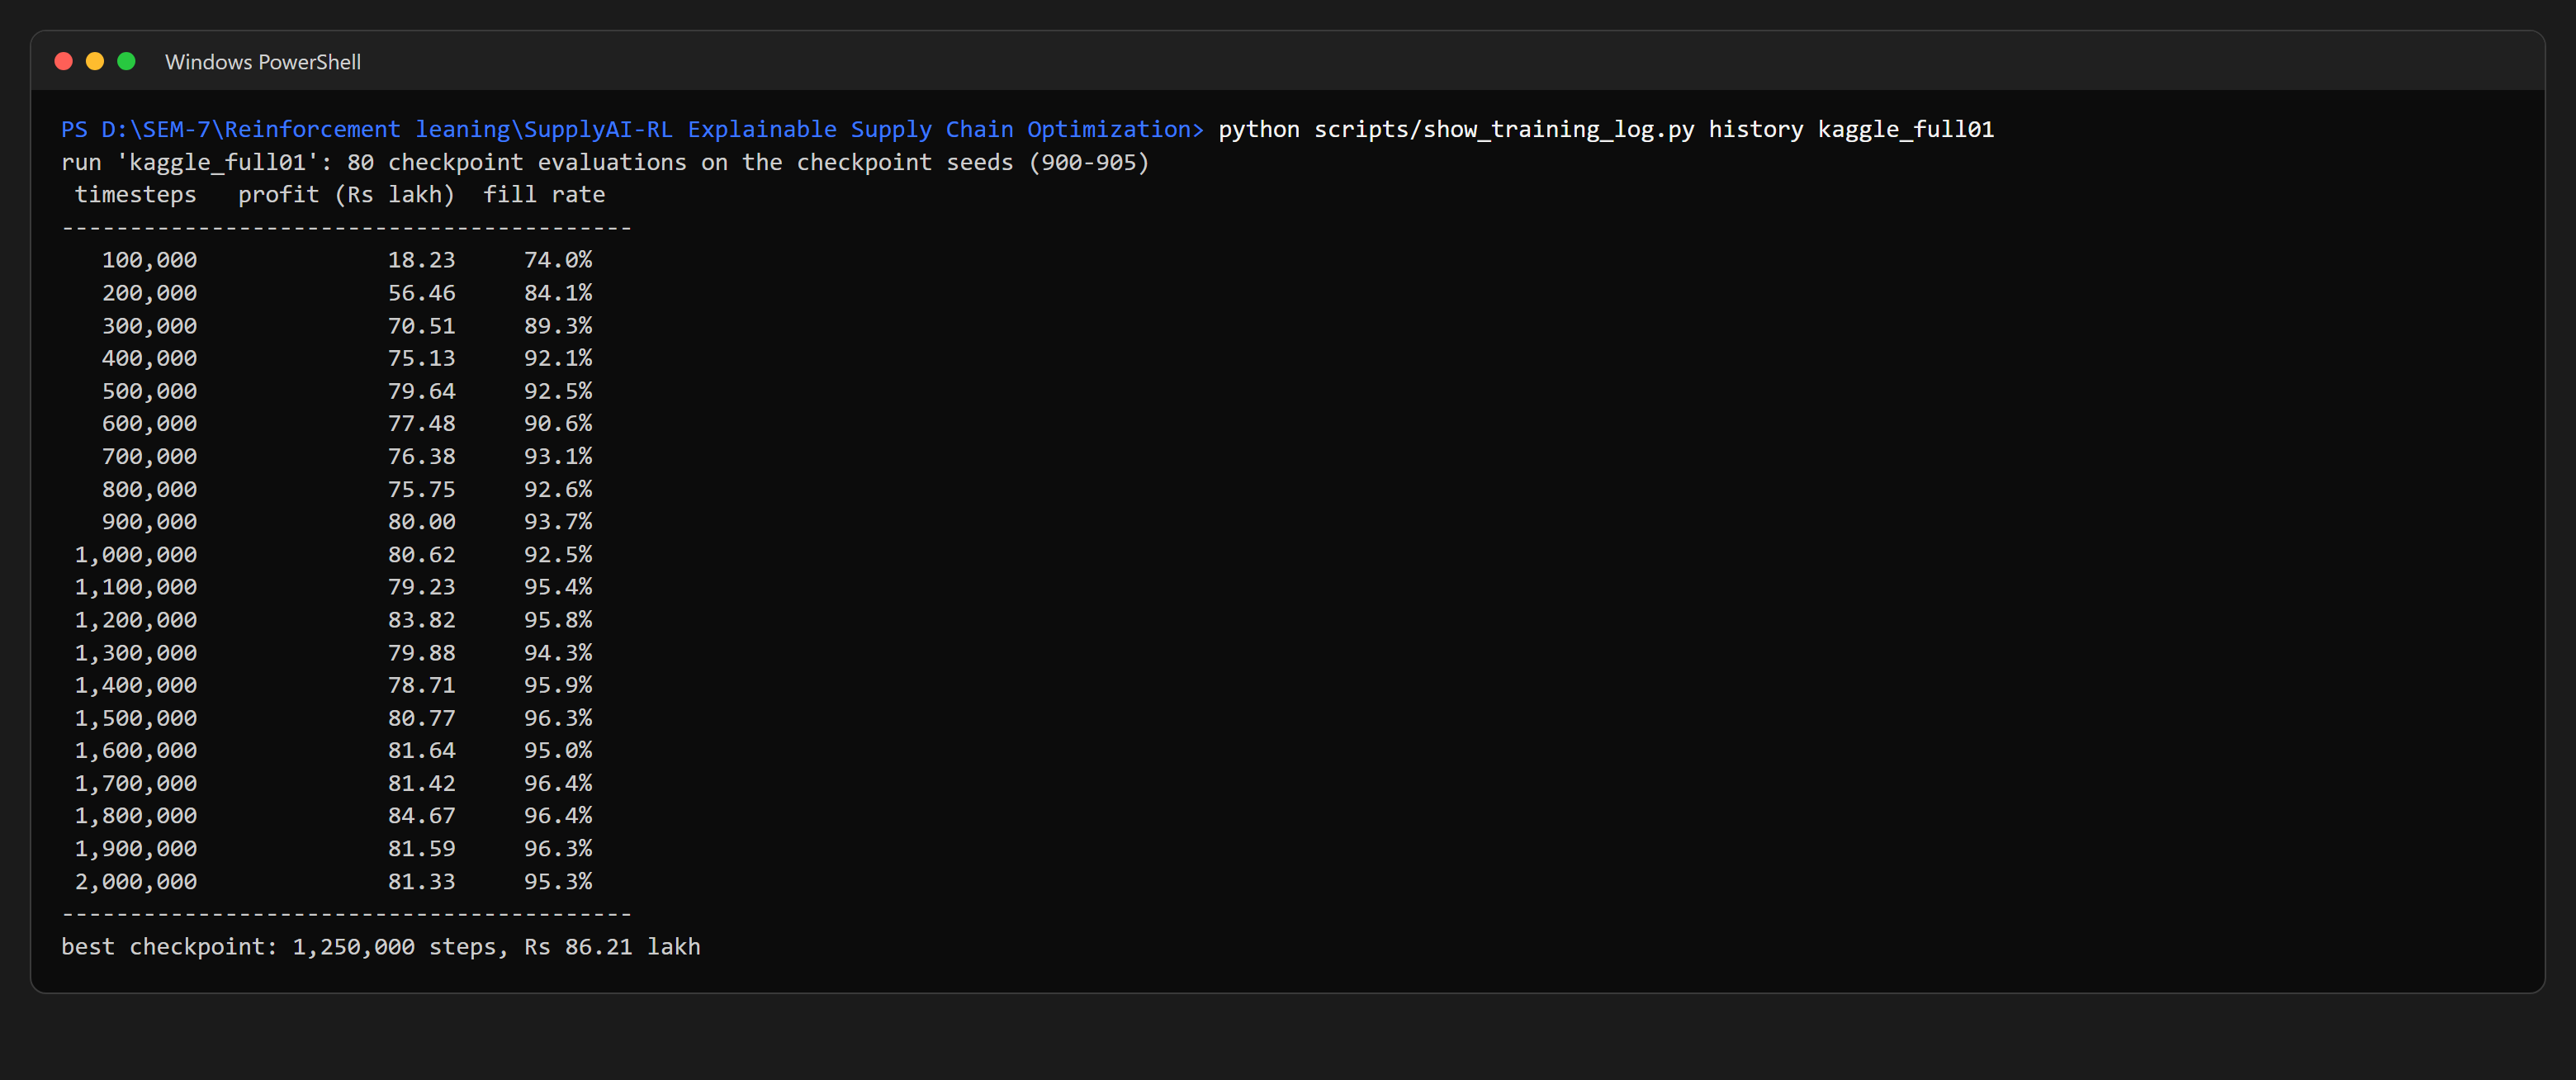
\includegraphics[width=0.9\textwidth]{figures/terminal_history.png}
\caption{Checkpoint evaluations of the tuned 2M-step agent, read from its saved
training history (profit per 180-day run on the checkpoint seeds).}
\label{fig:term-hist}
\end{figure*}

\begin{figure*}[t]
\centering
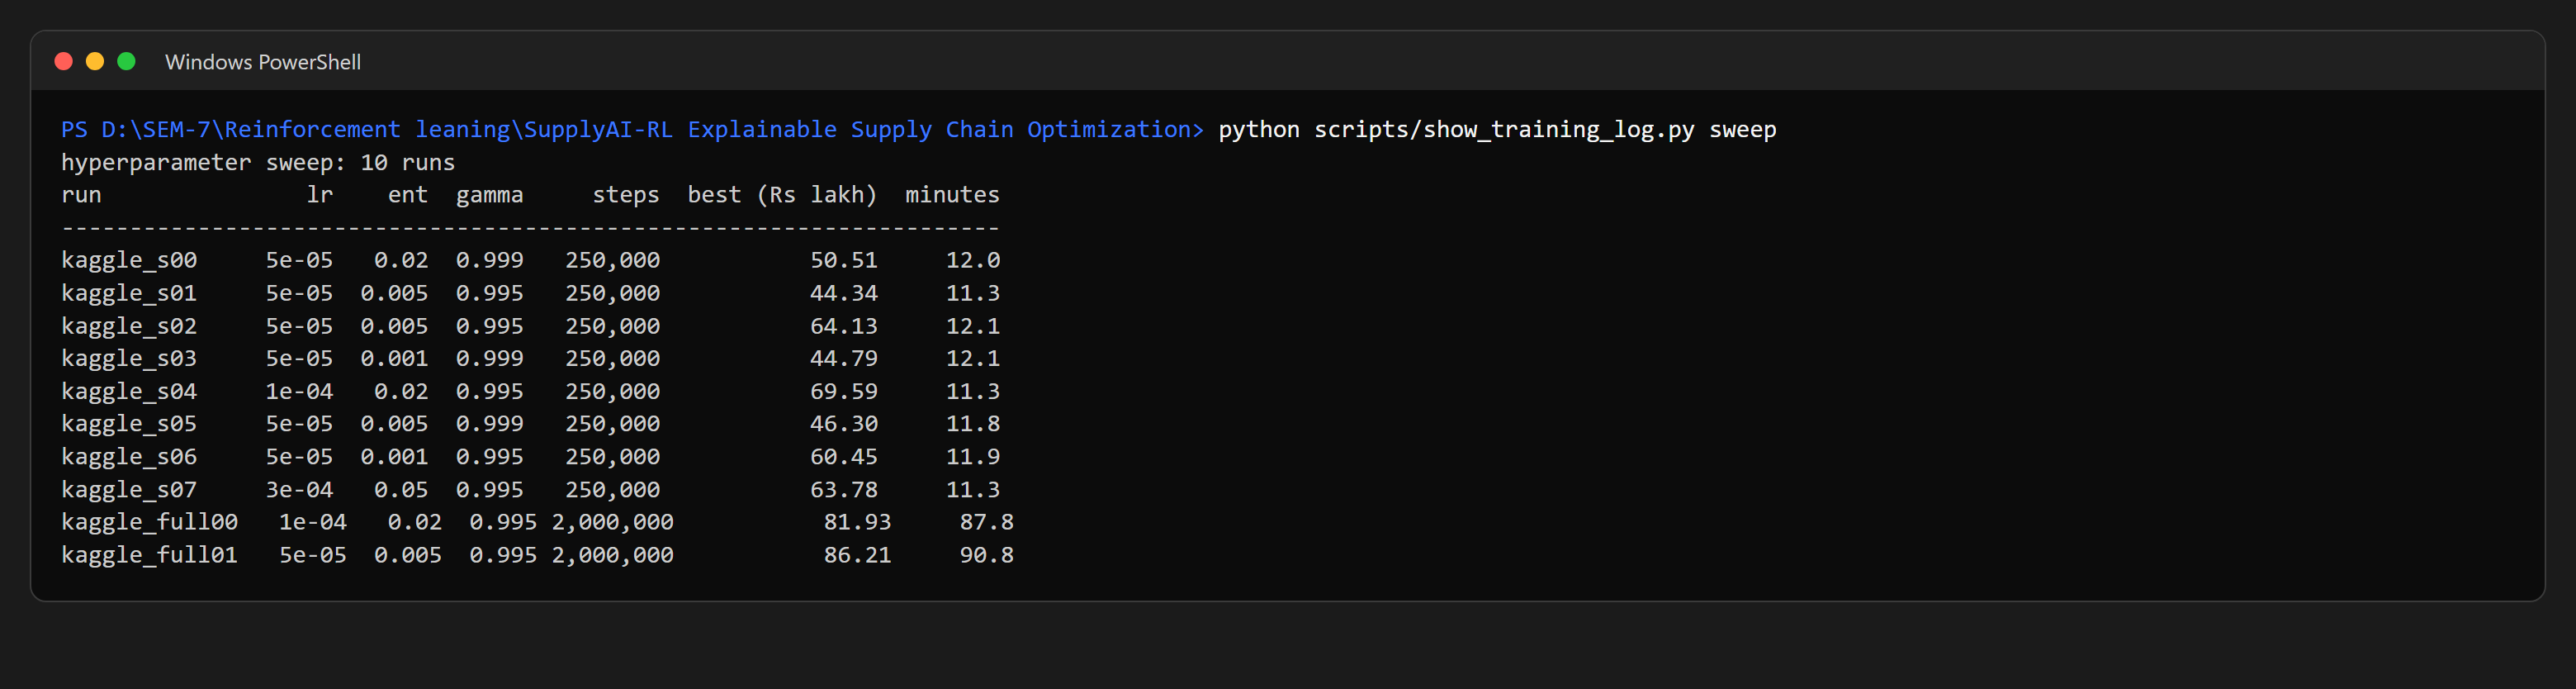
\includegraphics[width=0.9\textwidth]{figures/terminal_sweep.png}
\caption{Summary of the 8-configuration hyperparameter search, read from the
saved sweep results.}
\label{fig:term-sweep}
\end{figure*}

\paragraph{Statistics.}
We compare methods with paired $t$-tests on the per-seed differences ($n=30$)
and report the 95\% interval of the mean difference.

% ----------------------------------------------------------------- 6 results
\section{Results}

\subsection{Main Comparison}

Table~\ref{tab:main} and Figure~\ref{fig:policies} compare all methods on the
30 held-out seeds. The best classical policy, forecasting with safety stock,
earns \Rs 87.8\lakh{}. The tuned agent earns \Rs 79.7\lakh{}, or
\textbf{90.8\%} of that. The difference of \Rs 8.1\lakh{} is statistically
clear (paired $t=-6.45$, $n=30$, $p<0.001$, 95\% CI 5.5 to 10.6\lakh{}), and the
classical policy comes out ahead on 26 of the 30 seeds. The agent does beat two
of the four classical policies, EOQ and $(s,S)$. A shop with no system would
simply order the same amount every day. Compared with that, the engine raises
profit from \Rs 53.3\lakh{} to \Rs 87.8\lakh{} (+65\%) and wins on all 30
seeds. The agent beats the fixed order on 29 of 30.

\begin{table*}[t]
\centering\small
\begin{tabular}{lccccc}
\toprule
Method & Profit (\Rs lakh) & Std & Fill rate & Fees (\Rs lakh) & Stockout (\Rs lakh) \\
\midrule
Forecast + safety stock & \textbf{87.8} & 4.6 & 97.9\% & 2.9 & 6.1 \\
Newsvendor              & 86.2 & 4.4 & 98.0\% & 3.4 & 7.4 \\
\textbf{RL agent, tuned, 2M steps} & \textbf{79.7} & 5.5 & 95.1\% & 5.8 & 9.2 \\
RL agent, 2nd config, 2M steps     & 77.0 & 5.4 & 93.6\% & 7.1 & 10.5 \\
EOQ + reorder point     & 75.9 & 7.4 & 96.8\% & 2.8 & 10.5 \\
RL agent, untuned, 1M steps        & 74.8 & 5.8 & 94.3\% & 7.4 & 11.0 \\
$(s,S)$ policy          & 73.9 & 7.1 & 94.9\% & 3.1 & 16.5 \\
Constant order (no system)         & 53.3 & 13.4 & 92.3\% & 3.5 & 29.0 \\
RL agent, no masking, 1M steps     & 23.7 & 9.0 & 94.8\% & 14.7 & 11.3 \\
\bottomrule
\end{tabular}
\caption{Mean profit per 180-day run over 30 held-out seeds (500--529). Std is
the spread across seeds. All methods face the same customers and delays on each
seed. Rupee amounts use 1 GBP = \Rs 105.}
\label{tab:main}
\end{table*}

\begin{figure}[t]
\centering
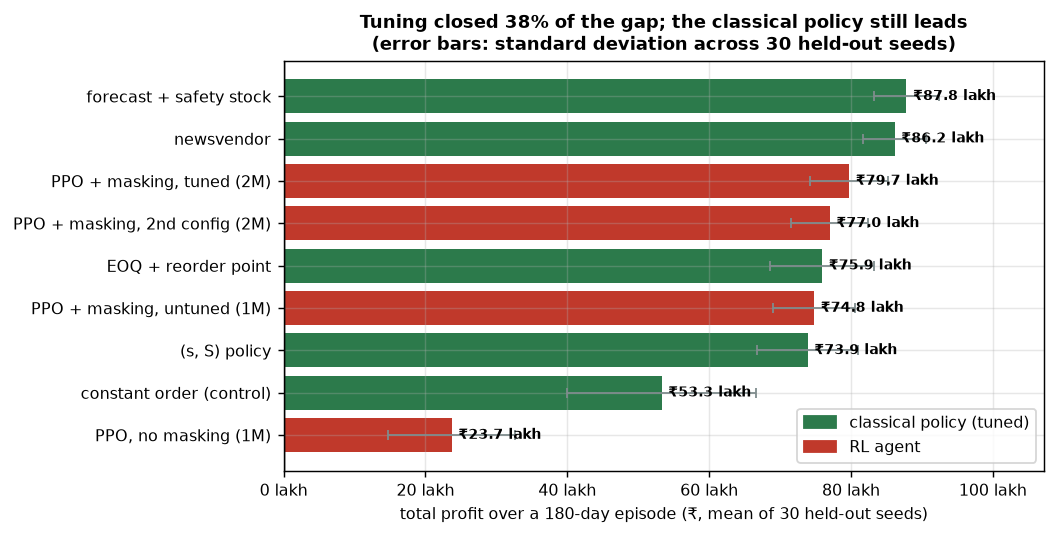
\includegraphics[width=\columnwidth]{figures/05_policy_comparison.png}
\caption{Profit of every method on the 30 held-out seeds. Green bars are
classical policies and red bars are RL agents. Error bars show the standard
deviation across seeds.}
\label{fig:policies}
\end{figure}

\subsection{Ablation: What Each Step Added}

Table~\ref{tab:steps} separates the two improvements. Action masking made by far
the biggest difference, about $3\times$. Without it the agent spends most of its
training finding out that some choices are pointless. Tuning and longer
training then closed 38\% of the remaining gap, taking it from \Rs 13.0\lakh{}
down to \Rs 8.1\lakh{}. The learning curves are in Figure~\ref{fig:curves}.

\begin{table}[t]
\centering\small
\setlength{\tabcolsep}{3pt}
\begin{tabular}{lccc}
\toprule
Step & Train & Test & Gap \\
\midrule
PPO, no masking     & 24.9 & 23.7 & $-64.1$ \\
+ action masking    & 76.4 & 74.8 & $-13.0$ \\
+ tuning, 2M steps  & 86.2 & 79.7 & $\mathbf{-8.1}$ \\
\bottomrule
\end{tabular}
\caption{Profit in \Rs lakh. Train: checkpoint seeds (900--905). Test: held-out
seeds (500--529). Gap: test profit minus the best classical policy.}
\label{tab:steps}
\end{table}

\begin{figure}[t]
\centering
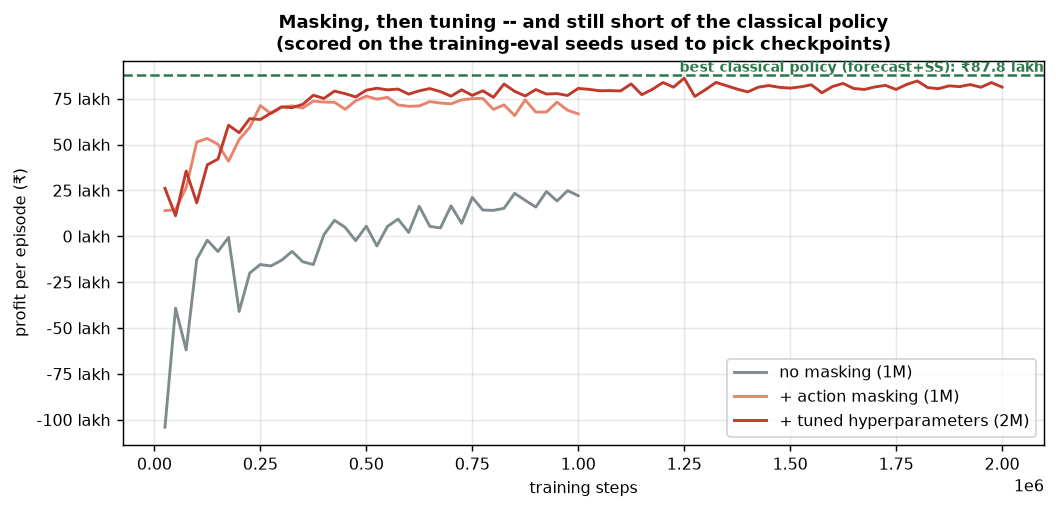
\includegraphics[width=\columnwidth]{figures/06_training_curves.png}
\caption{Learning progress on the checkpoint seeds. This shows how training
went. The reported scores come from the held-out seeds.}
\label{fig:curves}
\end{figure}

\subsection{Robustness to LLM-Generated Crises}

Table~\ref{tab:robust} scores each method on 10 normal seeds and on 6
held-out crisis sets that the agents never trained on. Every method loses more
than a third of its profit. The tuned agent never saw a crisis during
training, yet it has the highest crisis profit and the smallest drop among the
agents.

\begin{table}[t]
\centering\small
\setlength{\tabcolsep}{3pt}
\begin{tabular}{lccc}
\toprule
Method & Normal & Crisis & Drop \\
\midrule
Forecast + safety stock & 87.4 & 53.7 & $-38.6\%$ \\
\textbf{RL, tuned}      & 80.4 & \textbf{50.7} & $\mathbf{-37.0\%}$ \\
RL, untuned (control)   & 73.8 & 38.8 & $-47.5\%$ \\
RL, crisis-trained      & 66.0 & 38.9 & $-41.1\%$ \\
\bottomrule
\end{tabular}
\caption{Profit in \Rs lakh on normal seeds and on 6 unseen LLM-generated
crises.}
\label{tab:robust}
\end{table}

\textbf{Training on crises did not help.} The crisis-trained agent earns
\Rs 38.9\lakh{} in a crisis, against \Rs 38.8\lakh{} for the control, and it
gave up \Rs 7.7\lakh{} of normal profit to get there. Its smaller percentage
drop is misleading, because it starts lower and so has less to lose. The
difference is not significant ($t=+1.69$, $n=30$). This is why we show the drop
next to the actual profit.

\subsection{Explainer Accuracy}

We scored 30 real decisions (6 days $\times$ 10 products), shown in
Table~\ref{tab:explainer}. The LLM answered every call once retries were
allowed. In five of the 30 raw outputs there was a number the simulator never
produced. They read fluently, and a buyer would probably not have noticed. The
check caught all five and showed the template instead, so every explanation the
user saw was correct and complete. Without the check, about one explanation in
six would have carried a made-up figure.

\begin{table}[t]
\centering\small
\begin{tabular}{lc}
\toprule
Measure & Result \\
\midrule
LLM answered (after retries) & 100\% \\
Only real numbers (raw output) & 83\% (25/30) \\
Complete & 100\% \\
\textbf{Raw model accuracy} & \textbf{83\%} \\
\textbf{Delivered accuracy} & \textbf{100\%} \\
Length & 2.9 sentences, 58 words \\
\bottomrule
\end{tabular}
\caption{Explainer results on 30 decisions. Raw accuracy means all numbers were
real and the key details present, before the check. Delivered accuracy is what
the user saw.}
\label{tab:explainer}
\end{table}

Our first version of this metric only scored outputs that had already passed the
check. It reported 100\% for a model that invented numbers in 17\% of cases,
which told us nothing about the model, so we now report both figures.

% ------------------------------------------------------------- 7 error
\section{Error Analysis}

Where does the \Rs 8.1\lakh{} gap come from? Figure~\ref{fig:trace} shows one
traced run, and the averages in Table~\ref{tab:main} agree with it.

\begin{itemize}
  \item \textbf{Ordering fees.} The agent pays \Rs 5.8\lakh{} against
    \Rs 2.9\lakh{} for the best classical policy. It spreads its orders over
    all three suppliers. In the traced run it placed 719 orders and the
    classical policy placed 323, almost all with the cheap supplier.
  \item \textbf{Fill rate.} It is 95.1\% against 97.9\%. The agent runs out of
    stock more often, which costs about \Rs 3\lakh{} extra in penalties.
  \item \textbf{Overflow.} Only the RL agents have zero overflow loss. They
    learned the shared-warehouse limit, while every classical policy wastes
    some goods.
\end{itemize}

We think the reason for the fee gap is that the agent cannot observe its own
history. None of the 88 inputs says how long ago it last ordered, how much it
has paid in fees, or which supplier it used last. So it pays double and has no
way to notice. This is about what the agent can see, so more tuning would not
fix it. Adding a few history features per product looks like the most
promising change, but we have not tried it yet.

\begin{figure*}[t]
\centering
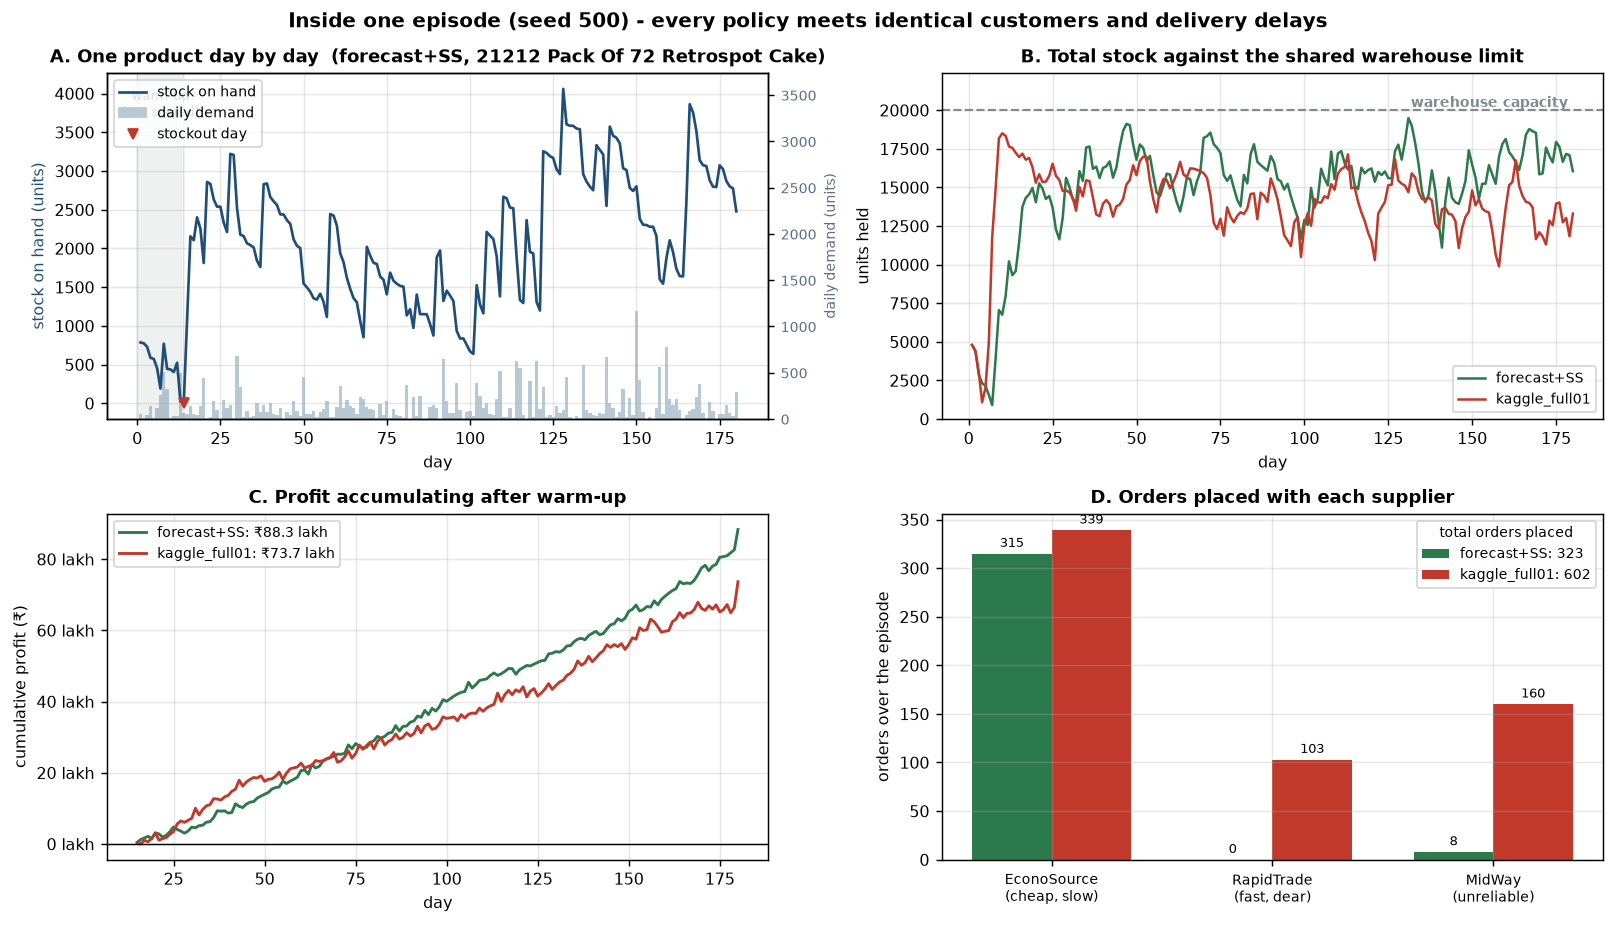
\includegraphics[width=0.85\textwidth]{figures/07_simulator_trace.png}
\caption{One run in the simulator: stock against demand for one product,
warehouse fill, cumulative profit, and the supplier mix (panel D).}
\label{fig:trace}
\end{figure*}

% ---------------------------------------------------- 8 efficiency / deploy
\section{Efficiency and Deployment}

Everything was trained on ordinary hardware. A 1M-step run takes about 48
minutes on a laptop CPU, and each 2M-step run took about 1.5 hours on Kaggle.
Training on crises costs roughly twice as much per step as normal training (we
measured 156 steps per second). We did not measure inference speed or memory
use.

Our results point to shadow mode, which is how the dashboard works. The tuned
classical policy is the engine a buyer would run. The agent runs beside it, and
its decisions are logged and scored but not carried out. The explainer covers
whichever decision is on screen. If the challenger beats the engine steadily on
live data, it could then be promoted. Several things are still missing before
real use: handling of new products with no history, limits on order value, an
audit trail, a live data feed, and a signal that tells a human to take over
when the system is unsure.

% --------------------------------------------------------- 9 limitations
\section{Limitations}

The first two matter most.

\paragraph{Invented suppliers.}
Lead times, reliability and fees were set by hand to cover the usual
trade-off. No public dataset records them, so the rupee values should be read as
relative comparisons and not as forecasts.

\paragraph{Unequal difficulty in crisis training.}
The crisis-trained agent had a harder task with the same number of steps, so
part of its weaker result may come from under-training and not from the method.

\paragraph{Explainer sample.}
We tested 30 decisions with one model setup and one seed. The explainer
restates computed facts. It does not describe how the network reasons, and we
do not claim that it does.

\paragraph{One shop, ten products.}
Other product categories, larger ranges and other cost structures were not
tested.

\paragraph{Free LLM endpoints.}
Free models are rate-limited, so an explanation can take up to a minute and
sometimes falls back to the template.

% -------------------------------------------------------- 10 broader impact
\section{Broader Impact}

We would not deploy the agent today, because it earns less than a simpler
method and is no more robust. We would use it only as a scored challenger.
There is one more risk to name. An explanation that reads smoothly can make a
wrong decision look right. That is why the numbers are checked, and why we call
the explanation a restatement of facts and not a reason. Because the suppliers
are invented, the rupee figures are best read as comparisons inside one
simulator.

% ------------------------------------------------------------ 11 conclusion
\section{Conclusion}

A MaskablePPO agent reaches 90.8\% of the profit of the best tuned classical
policy on 30 held-out seeds. It beats two of the four classical policies and
beats a fixed daily order on 29 of 30 seeds, but the best classical policy still
wins by \Rs 8.1\lakh{} per run ($t=-6.45$). So the idea that RL would adapt
better than a tuned formula did not hold up, either on normal days or in a
crisis. What we can say with confidence comes from how we tested it. The
baselines were tuned, the test seeds were kept separate, the crisis-trained
agent was tested on crises it had never seen, and the percentage drop was shown
next to the actual profit. Action masking and tuning each helped by a
measurable amount, and training on crises did not. The explainer is accurate
only because its output is checked: 83\% before the check and 100\% after.

The error analysis suggests the next step. The gap comes from fees caused by
splitting orders across suppliers, and the agent cannot see its own ordering
history. Giving it that history and repeating the same evaluation is the
experiment most likely to change the main result.

% -------------------------------------------------------------- references
\begin{thebibliography}{99}\small
\setlength{\itemsep}{1pt}

\bibitem{ppo} J.~Schulman, F.~Wolski, P.~Dhariwal, A.~Radford, and
O.~Klimov. Proximal policy optimization algorithms. arXiv:1707.06347, 2017.

\bibitem{masking} S.~Huang and S.~Ontañón. A closer look at invalid action
masking in policy gradient algorithms. In \emph{FLAIRS-35}, 2022.

\bibitem{gijsbrechts} J.~Gijsbrechts, R.~N.~Boute, J.~A.~Van~Mieghem, and
D.~Zhang. Can deep reinforcement learning improve inventory management?
\emph{Manufacturing \& Service Operations Management}, 2022.

\bibitem{boute} R.~N.~Boute, J.~Gijsbrechts, W.~van Jaarsveld, and
N.~Vanvuchelen. Deep reinforcement learning for inventory control: A roadmap.
\emph{European Journal of Operational Research}, 2022.

\bibitem{beer} A.~Oroojlooyjadid, M.~Nazari, L.~V.~Snyder, and M.~Takáč.
A deep Q-network for the beer game. \emph{Manufacturing \& Service Operations
Management}, 2022.

\bibitem{chen} D.~Chen, S.~L.~Sain, and K.~Guo. Data mining for the online
retail industry. \emph{Journal of Database Marketing \& Customer Strategy
Management}, 2012.

\bibitem{sb3} A.~Raffin et al. Stable-Baselines3: Reliable reinforcement
learning implementations. \emph{JMLR}, 22(268), 2021.

\bibitem{uci} UCI Machine Learning Repository. Online Retail II.
\url{https://archive.ics.uci.edu/dataset/502}.

\end{thebibliography}

\end{document}
